
\section{Simulation Setup and Parameters}

The experimental evaluation is conducted within the custom-built OpenAI Gymnasium environment described in Chapter 3. To ensure realism, the microgrid parameters are calibrated to match the specifications of a standard residential battery system, specifically modeling a Tesla Powerwall 2. The battery has a total energy capacity of 13.5 kWh with a usable depth of discharge of 90\%, implying a minimum state of charge of 10\%. The inverter is rated at 5.0 kW for both continuous charging and discharging. The round-trip efficiency is modeled as 90\%, which is decomposed into a 95\% efficiency for charging and 95\% for discharging.

The simulation utilizes real-world electricity consumption and production data. The dataset is partitioned into training and testing subsets to evaluate the generalization capability of the agents. The best-performing day (highest solar generation) is selected for the primary evaluation to stress-test the control strategies under conditions with substantial arbitrage opportunity.

Both the Soft Actor-Critic (SAC) and Proximal Policy Optimization (PPO) agents are trained for a total of 200,000 time steps. This duration was empirically determined to be sufficient for the policy to converge to a stable solution. The SAC agent uses a learning rate of $3 \times 10^{-4}$, while the PPO agent is configured with a lower learning rate of $3 \times 10^{-4}$ and a larger rollout buffer of 4,096 steps to improve gradient estimates. The Robust SAC (R-SAC) agent employs a more conservative learning rate of $1 \times 10^{-4}$ with a larger replay buffer of 100,000 transitions. For robustness training, domain randomization is applied with a noise level of 30\% and a temporal correlation factor of 0.9, as defined in Section 4.3.

\begin{table}[h]
    \centering
    \caption{Key Simulation Parameters}
    \label{tab:sim_params}
    \begin{tabular}{lc}
    \toprule
    \textbf{Parameter} & \textbf{Value} \\
    \midrule
    Battery Capacity ($E_{max}$) & 13.5 kWh \\
    Max Power ($P_{max}$) & 5.0 kW \\
    Min State of Charge & 10 \% \\
    Charging Efficiency & 95 \% \\
    Discharging Efficiency & 95 \% \\
    Peak Power Threshold & 10.0 kW \\
    Peak Penalty Rate & \$0.50/kW \\
    Degradation Cost & \$0.02/kWh \\
    Forecast Horizon & 24 Hours \\
    Time Step ($\Delta t$) & 1 Hour \\
    Training Steps & 200,000 \\
    Evaluation Episodes & 100 \\
    SAC Learning Rate & $3 \times 10^{-4}$ \\
    PPO Learning Rate & $3 \times 10^{-4}$ \\
    R-SAC Learning Rate & $1 \times 10^{-4}$ \\
    Discount Factor ($\gamma$) & 0.99 \\
    SAC Buffer Size & 50,000 \\
    R-SAC Buffer Size & 100,000 \\
    \bottomrule
    \end{tabular}
\end{table}

\begin{figure}[h]
    \centering
    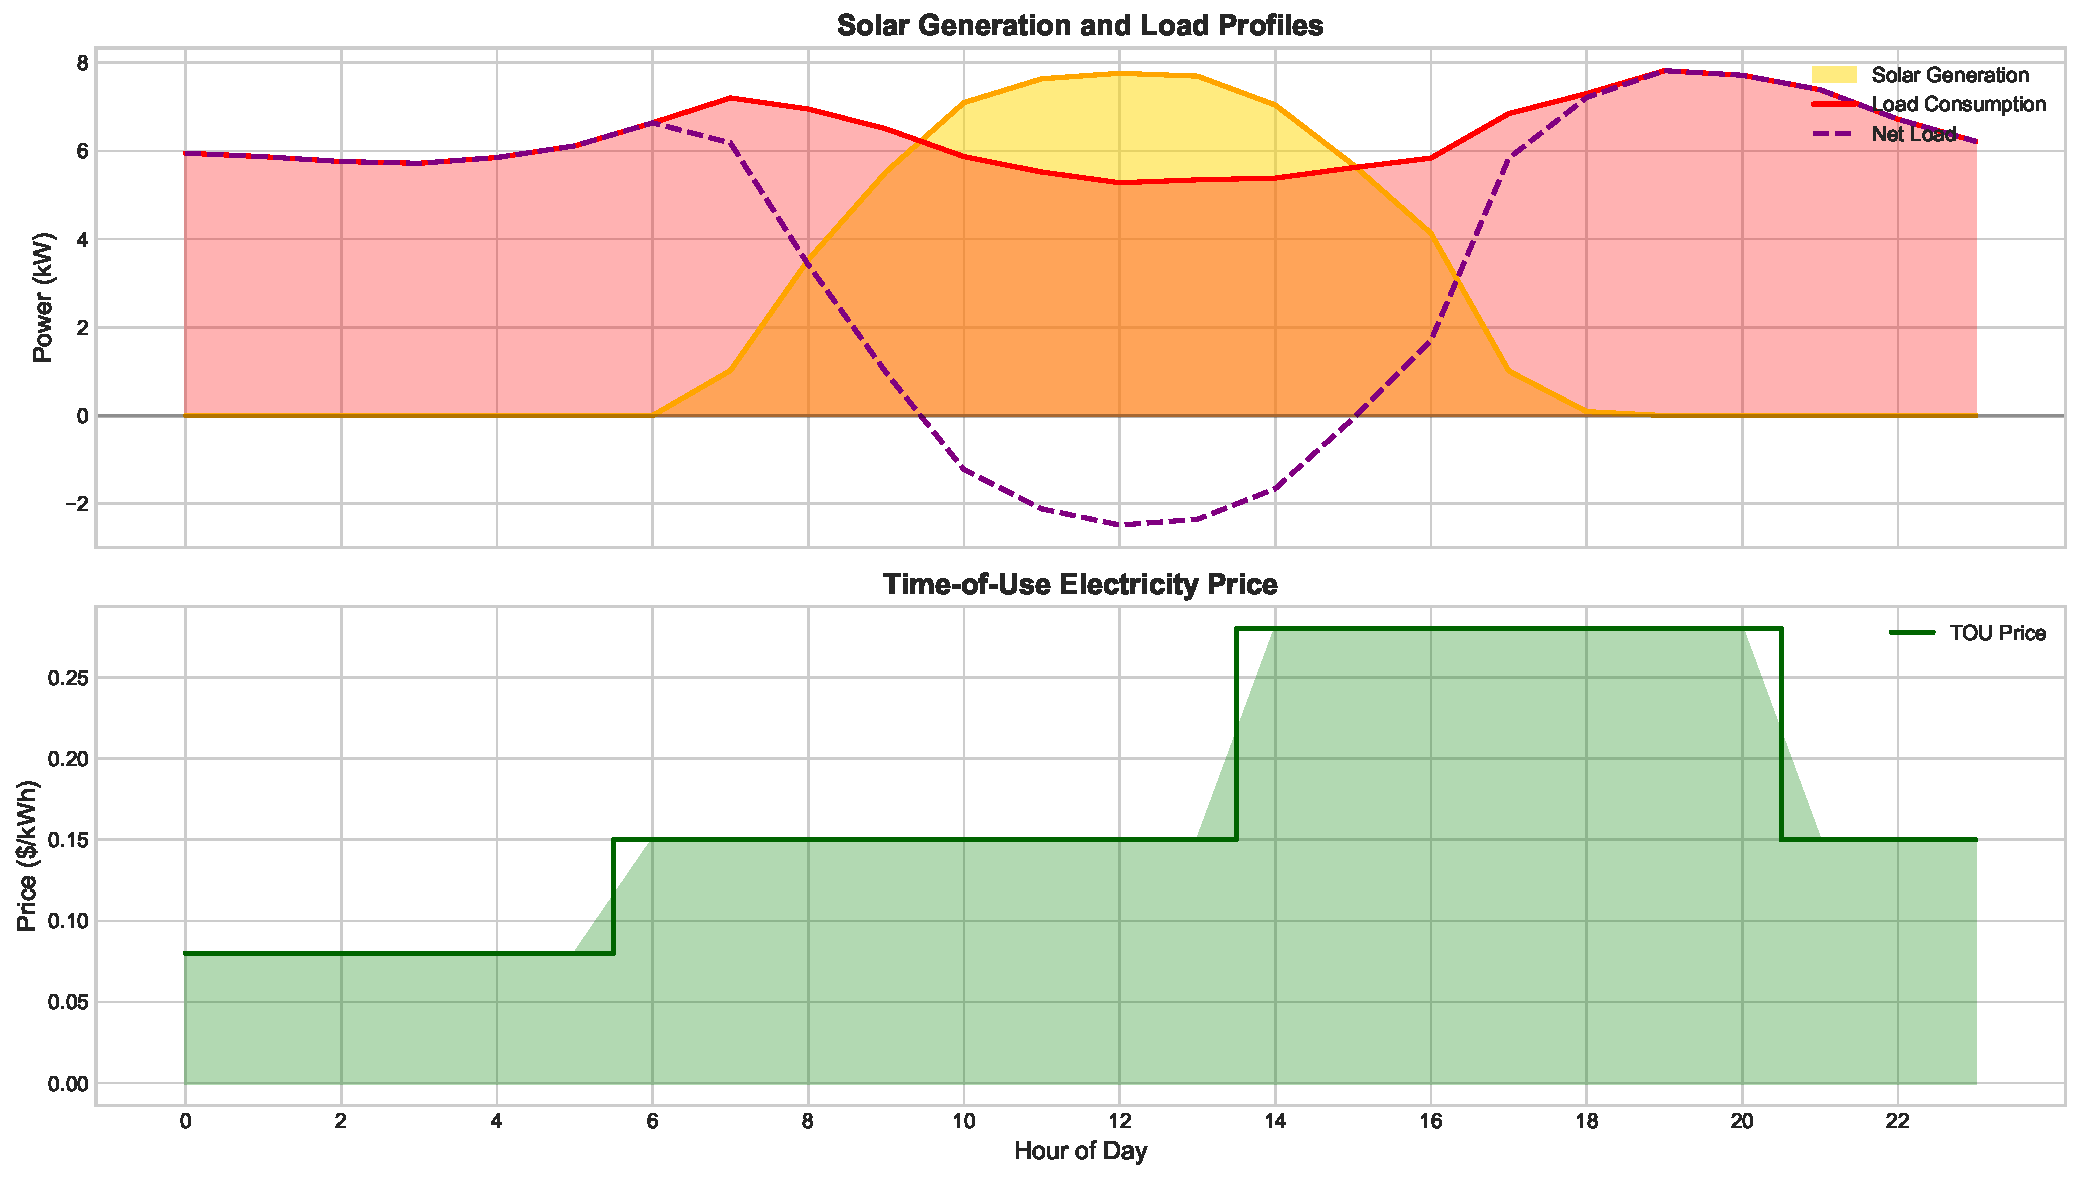
\includegraphics[width=1\textwidth]{Pages/fig/11_profiles.pdf}
    \caption{Daily profiles of Solar Generation (kW), Load Demand (kW), and Time-of-Use Electricity Prices (\$/kWh) used in the simulation.}
    \label{fig:profiles}
\end{figure}